\documentclass[journal,12pt,twocolumn]{IEEEtran}
\usepackage{amsmath}
\usepackage{amssymb}
\usepackage{enumerate}
\usepackage[utf8]{inputenc}
\usepackage{multicol}
\usepackage{gensymb}
\usepackage{mathtools}
\usepackage{physics}
\usepackage{graphicx}
%\usepackage{iithtlc}
%\usepackage{iithquiz}

%\graphicspath{ {/home/theresh/Desktop/DSP} }



\newcommand\Mycomb[2][^n]{\prescript{#1\mkern-0.5mu}{}C_{#2}}


\begin{document}
\providecommand{\qfunc}[1]{\ensuremath{Q\left(#1\right)}}
\providecommand{\sbrak}[1]{\ensuremath{{}\left[#1\right]}}
\providecommand{\lsbrak}[1]{\ensuremath{{}\left[#1\right.}}
\providecommand{\rsbrak}[1]{\ensuremath{{}\left.#1\right]}}
\providecommand{\brak}[1]{\ensuremath{\left(#1\right)}}
\providecommand{\lbrak}[1]{\ensuremath{\left(#1\right.}}
\providecommand{\rbrak}[1]{\ensuremath{\left.#1\right)}}
\providecommand{\cbrak}[1]{\ensuremath{\left\{#1\right\}}}
\providecommand{\lcbrak}[1]{\ensuremath{\left\{#1\right.}}
\providecommand{\rcbrak}[1]{\ensuremath{\left.#1\right\}}}

\title{
\logo{Gate problems in DSP
%\logo{Gate problems in DSP}{\includegraphics[scale=0.3]{tlc2.eps}}{}{}
}
}

%\maketitle

\begin{abstract}
These problems have been selected from
GATE question papers and can be used for conducting
tutorials in courses related to the course Digital Signal Processing in practice.
\end{abstract}


\begin{enumerate}
\setlength\itemsep{2em}

\item The inverse Laplace trasform of H(s)=$\frac{s+3}{s^2+2s+1}$ for t$\geq$0
\begin{enumerate}[(A)]

\setlength\itemsep{0.5em}

\item $ 3te^{-t}+e^{-t}  $
\item $3e^{-t}$

\item $ 2te^{-t}+e^{-t}  $

\item $ 4te^{-t}+e^{-t}  $

\end{enumerate}

\item A system Transfer Function is H(s)=$\frac{a_1s^2+b_1s+c_1}{a_2s^2+b_2s+c_2}$. If $a_1=b_1=0$ and all other coefficients are positive, the transfer function represents a-
\begin{enumerate}[(A)]

\setlength\itemsep{0.5em}

\item $ low pass filter $
\item $High Pass filter$

\item $ band pass filter  $

\item $ notch filter$

\end{enumerate}

\item The symbols, a and T, represent positive quantities, and u(t) is the unit step function. Which one of the following impulse responses is NOT the output of a causal linear time-invariant system-

\begin{enumerate}[(A)]

\setlength\itemsep{0.5em}

\item $ e^{at}u(t)$
\item $ e^{-a(t+T)}u(t)$

\item $ 1+e^{-at}u(t) $

\item $ e^{-a(t-T)}u(t) $

\end{enumerate}

\item A periodic function f(t) with a period of $2\pi$ is represented as its Fourier series, 
\begin{equation}
    f(t)=a_0+\sum _{n=1 }^{\infty }a_n\cos nt+\sum _{n=1 }^{\infty }a_n\sin nt
\end{equation}
if
\[
	f(t)=\begin{cases}
		A\sin t, &  {0\leq t \leq \pi}  \\
		0, &   \pi \leq t \leq 2\pi ,
	\end{cases}
\] 
the Fourier series coefficients $a_1$ and $b_1$ of f(t) are-
\begin{enumerate}[(A)]

\setlength\itemsep{0.5em}

\item $ a_1=\frac{A}{\pi}; b_1=0$
\item $ a_1=\frac{A}{2}; b_1=0$

\item $ a_1=0; b_1=\frac{A}{\pi}$

\item $ a_1=0; b_1=\frac{A}{2}$

\end{enumerate}

\item  Let H(z) be the z-transform of a real-valued discrete-time signal h[n]. If $P(z)=H(z)H(\frac{1}{z})$ has a zero at $z=\frac{1}{2}+\frac{1}{2}j$, and P(z) has a total of four zeros, which one of the following plots represents all the zeros correctly?

\begin{figure}[!ht]
\begin{center}
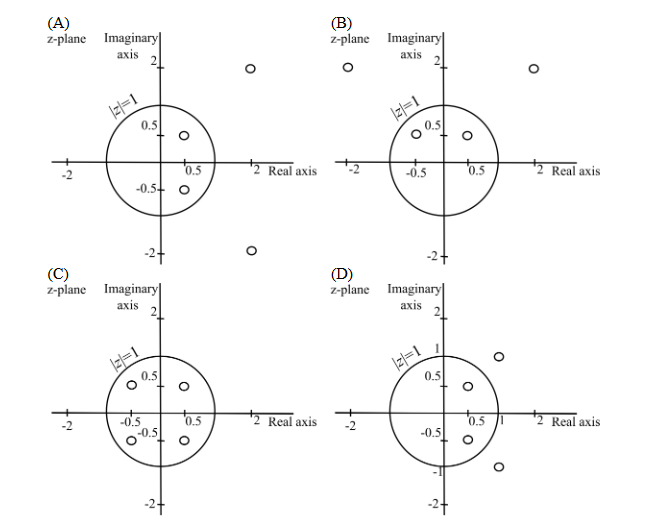
\includegraphics[width=1.2\columnwidth]{./EC_1}
\end{center}
%\captionof{Question}{}
\label{fig:EC_1}	
\end{figure}

\item Consider the signal f(t)=$1+2\cos{\pi t}+ 3\sin{(\frac{2\pi}{3})t} +4\cos{(\frac{\pi}{2}t+\frac{\pi}{4})}$ where t in seconds. Its Fundamental time period, in second is. \underline{\hspace{2cm}}


\item It is desired to find a three-tap causal filter which gives zero signal as an output to an input of the form
\begin{equation}
    x[n]=c_1e^{\frac{-j\pi n}{2}}+c_2e^{\frac{j\pi n}{2}}
\end{equation}
where $c_1$ and $c_2$ are arbitrary real numbers. The desired three-tap filter is given by
h[0]=1, h[1]=a, h[2]=b and h[n]=0 otherwise\\
What are the values of the filter taps a and b if the output is y[n]=0 for all n, when x[n] is as given above?

\begin{enumerate}[(A)]

\setlength\itemsep{0.5em}

\item $ a_1=1; b_1=1$
\item $ a_1=0; b_1=-1$

\item $ a_1=-1; b_1=1$

\item $ a_1=0; b_1=1$

\end{enumerate}

\item Let h[n] be  a length-7 discrete-time finite impulse response filter, given by: \\h[0]=4, h[1]=3, h[2]=2, h[3]=1\\
h[-1]=-3, h[-2]=-2,  h[-3]=-1\\
and h[n]=0 for $|n| \geq 4 $. A length-3 finite impulse response approximation g[n] of h[n] has to be obtained such that- \\
E(h,g)= ${\int_{-\pi}^{\pi}{(|H(e^{j\omega})|-|G(e^{j\omega})|)^2}d\omega }$ \\
is minimized, where $H(e^{j\omega})$ and $G(e^{j\omega})$  are the discrete-time Fourier transforms of h[n] and g[n],respectively. For the filter that minimizes E(h,g),  the value of 10g[-1]+g[1], rounded off to 2 decimal places, is \underline{\hspace{2cm}}


\item A discrete-time all-pass system has two of its poles at $0.25\angle 0^\circ$ and $2\angle 30^\circ $. Which one of the
following statements about the system is TRUE?
\begin{enumerate}[(A)]

\setlength\itemsep{0.5em}

\item  It has two more poles at $ 0.5\angle 30^\circ$ and $4\angle 0^\circ  $
\item  It is stable only when the impulse response is two-sided.

\item  It has constant phase response over all frequencies.

\item It has constant phase response over the entire
z-plane.

\end{enumerate}

\item Let x(t) be a periodic function with period T=10. The Fourier series coefficients for this series are denoted by $a_k$, that is-\\
$x(t)=\sum _{k=-\infty }^{\infty }a_k e^{\frac{jk2\pi t}{T}}$ \\
The same function x(t) can also be considered as a periodic function with period T'=40. Let $b_k$ be the Fourier series coefficients when period is taken as T'. If $\sum _{k=-\infty }^{\infty } |a_k|$ =16. Then $\sum _{k=-\infty }^{\infty } |b_k|$ is equal to-
\begin{enumerate}[(A)]

\setlength\itemsep{0.5em}

\item 256
\item 64

\item 16

\item 4

\end{enumerate}

\item Let X[k]=k+1, $0 \leq k \leq$ 7 be a 8-point DFT of a sequence x[n],
where \\ X[k]=$\sum _{n=0 }^{N-1 } x[n] e^{\frac{-j2\pi nk}{N}}$
The value (correct to two decimal places) of $\sum _{n=0 }^{3 } x[2n]$ is  \underline{\hspace{2cm}}

\item Let the input be u and the output be y of a system and the other parameters are real constants. Identify which among the following system is not a linear system
\begin{enumerate}[(A)]

\setlength\itemsep{0.5em}

\item $\dv[3]{y}{t}+a_1\dv[2]{y}{t}+a_2\dv{y}{t}+a_3y=b_3u+b_2\dv{u}{t}+b_1\dv[2]{u}{t}$ (with initial rest conditions)
\item $y(t)={\int_{0}^{t}e^{\alpha(t-\tau)}\beta u(\tau)}d\tau$

\item $y=au+b$

\item $y=au$

\end{enumerate}
\item Let f be the real valued function of a real variable defined $f(x)=x-[x]$, where [x] denotes the largest integer less than or equal to x. The value of $ {\int_{0.25}^{1.25} f(x) }dx $ is - \underline{\hspace{2cm}}

\item Consider the two continuous-time signals defined below: 
\[
	x_1(t)=\begin{cases}
		|t|, &  {-1\leq t \leq 1}  \\
		0, &   otherwise,
	\end{cases}
\] 
\[
	x_2(t)=\begin{cases}
		1-|t|, &  {-1\leq t \leq 1}  \\
		0, &   otherwise,
	\end{cases}
\]
These signals are sampled with a sampling period of T=0.25 seconds to obtain discrete-time signals $x_1[n]$ and $x_2[n]$, respectively.Which one of the following statements is true ?

\begin{enumerate}[(A)]

\setlength\itemsep{0.5em}

\item The energy of $x_1[n]$ is greater than the energy of $x_2[n]$
\item The energy of $x_2[n]$ is greater than the energy of $x_1[n]$

\item $x_![n]$ and $x_2[n]$ have equal energies.

\item Neither $x_1[n]$ nor $x_2[n]$ is a finite-energy signal.

\end{enumerate}


\item The signal energy of the continuous time signal
$x(t)=[(t-1)u(t-1)]-[(t-2)u(t-2)]-[(t-3)u(t-3)]+[(t-4)u(t-4)]$ is
\begin{enumerate}[(A)]

\setlength\itemsep{0.5em}

\item $\frac{11}{3}$
\item $\frac{7}{3}$

\item $\frac{1}{3}$

\item $\frac{5}{3}$

\end{enumerate}
\item The input x[n] and output y[n] of a discrete-time system are related as $y[n]=\alpha[n-1]+x[n]$. The condition on $\alpha$ for which the system is Bounded-Input Bounded-Output(BIBO) stable is-
\begin{enumerate}[(A)]

\setlength\itemsep{0.5em}

\item $|\alpha|< 1$
\item $|\alpha|=1$

\item $|\alpha|>1$

\item $|\alpha|< \frac{3}{2}$

\end{enumerate}
\item The output of a continuous-time system y(t) is related to input x(t) as $y(t)=x(t)+\frac{1}{2}x(t-1)$. If the Fourier transform of x(t) and y(t) are $X(\omega)$ and $Y(\omega)$ respectively, and $|X(0)|^2=4$, the value of $|Y(0)|^2$ is \underline{\hspace{2cm}}

\item A discrete-time signal $x[n]=e^{\frac{j5\pi n}{8}}+e^{\frac{j\pi n}{4}}$ is down-sampled to the signal $x_d[n]$ such that  $x_d[n] =x[4n]$. The fundamental period of the down-sampled signal $x_d[n]$ is \underline{\hspace{2cm}}

\item Two periodic signals $x(t)$ and $y(t)$ have the same fundamental period of 3 seconds. Consider the signal $z(t)=x(-t)+y(2t+1)$. The fundamental period of $z(t)$ in seconds is- 
\begin{enumerate}[(A)]

\setlength\itemsep{0.5em}

\item 1
\item 1.5

\item 2

\item 3

\end{enumerate}
\item Consider signal -
\[
	x(t)=\begin{cases}
		1, &  {-2\leq t \leq 2}  \\
		0, &   otherwise,
	\end{cases}
\]
Let $\delta(t)$ denote the unit impulse (Dirac-delta) function. The value of integral $ {\int_{0}^{5} 2x(t-3)\delta(t-4) }dt $ is-

\begin{enumerate}[(A)]

\setlength\itemsep{0.5em}

\item 2
\item 1

\item 0

\item 3

\end{enumerate}
\item The Fourier transform of a signal $x(t)$, denoted by $X(j\omega)$, is shown in the figure.
\begin{figure}[!ht]
\begin{center}
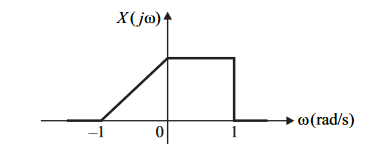
\includegraphics[width=1.2\columnwidth]{./gate_2}
\end{center}
%\captionof{}{}
\label{fig:gate_2}	
\end{figure}
Let $y(t)=x(t)+e^{jt}x(t)$. The value of Fourier transformof $y(t)$ evaluated at the angular frequency $\omega$= 0.5 rad/s is-
\begin{enumerate}[(A)]

\setlength\itemsep{0.5em}

\item 0.5
\item 1

\item 1.5

\item 2.5
\end{enumerate}
\item Let $y[n]=x[n]*h[n]$, where $*$ denotes convolution and x[n] and h[n] are two discrete time sequences. Given that the z-transform of $y[n]$ is $Y(z)=2+3z^{-1}+z^{-2}$, the z-transform of $p[n]=x[n]*h[n-2]$ is
\begin{enumerate}[(A)]

\setlength\itemsep{0.5em}

\item $2+3z+z^{-2}$
\item $3z+z^{-2}$

\item $2z^{2}+3z+1$

\item $2z^{-2}+3z^{-3}+z^{-4}$
\end{enumerate}
\item For the sequence $x[n]$= {1,-1,1,-1} with n=0,1,2,3 the DFT is computed as $X(k)=\sum _{k=0 }^{3} x[n]e^{\frac{-j2\pi nk}{4}} $, for k=0,1,2,3. The value of k for which X(k) is not zero is-
\begin{enumerate}[(A)]

\setlength\itemsep{0.5em}

\item 0
\item 1

\item 2

\item 3
\end{enumerate}

\item Unit step response of a linear time invariant (LTI) system is given by $y(t)=(1-e^{-2t})u(t)$. Assuming zero initial condition, the transfer function of the system is-
\begin{enumerate}[(A)]

\setlength\itemsep{0.5em}

\item $\frac{1}{s+1}$
\item $\frac{2}{(s+1)(s+2)}$

\item $\frac{1}{s+2}$

\item $\frac{2}{s+2}$
\end{enumerate}


\end{enumerate}

\end{document}
